\documentclass[10pt]{article}
\usepackage[margin=0.9in]{geometry}
\usepackage{amsmath,booktabs,hyperref,graphicx}
\title{Physical Action Effects in Dexterous Interaction Models:\\Measurement, Randomized Identification, and Task-Utility Prerequisites}
\author{Exploratory working manuscript, revision 4}
\date{1 October 2026}
\begin{document}
\maketitle
\begin{abstract}
We investigate whether physical action-effect information can support dexterous
decisions on an existing Inspire-hand simulation substrate. Initial physical,
contrast-learning and actuation-factorization screens fail their fixed gates.
Cold replay acquires interacting states but fails a strict pre-intervention
matching requirement. Prospective randomized assignment instead identifies
conditional-effect risk differences without asserting solver-state clones.
Archived predictors show no robust causal advantage on 3072 new windows; a
directly supervised contrast learner also fails on 3072 further windows.
Exploratory evidence from its factual control motivates a fresh randomized
closed-loop test with 3072 complete episodes. Greedy selection raises mean
object height by 2.60 mm versus the native actor, but retained success is
0.80\% versus 1.17\%, failing all utility gates. An independent label audit
finds that reference lift intervals last only 25--36 frames and end in return
to the table, while evaluation demands 45-step holding and full-episode nonreturn.
We retain this design limitation and freeze a separate synthetic holding-task
feasibility test. These exploratory results establish neither a new general
modeling method nor manipulation-policy improvement or journal readiness.
\end{abstract}

\section{Problem and relation to prior work}
An interaction model can fit common motion while failing to compare alternative actions.
Useful comparisons additionally require experiments capable of measuring physical
differences at the states in which actions are selected. We examine this prerequisite
before committing further resources to a policy. The repository provides self-trained
actors, geometric models and a DExplore simulation substrate \cite{xu2025}. Historical
policy audits are motivation rather than fresh evidence for this manuscript.

Shared particle actions and cross-embodiment world models already support planning
\cite{he2025}. Value-aware objectives \cite{farahmand2017}, predictor-level action
recovery \cite{qiu2026} and multi-step controllability representations \cite{rudolph2024}
are established. Contact-consistent replay and actuator residuals are also developed
by Contact-UAN \cite{fey2026}. Our small physical MLP studies do not reproduce these
systems or establish priority for their general principles. The present contribution
is an exploratory evidence record with frozen hypotheses and retained failures.

\section{Initial physical and contrast-learning screens}
Four panels combine actor seeds 286/287 with environment seeds 288/289, each with
32 environments for each of three airplane motions. A retrospective trigger schedules
one step after the first reference event where independent hand and object force
proxies are active. A one-step wrist-z action change requests a plus or minus 10-mm
PD target offset. This is a desired offset, not measured wrist travel. All subsequent
normalized actions and RNG schedules are replayed. Two zero arms measure repeated
process variation. Each object response subtracts its own actual pre-intervention
position. Pulse and repeat contrasts are summarized by vector RMS.

\begin{table}[h]
\centering
\begin{tabular}{lrr}
\toprule
Steps & Pulse RMS (mm) & Repeat RMS (mm)\\
\midrule
1 & 1.914 & 0.000\\
2 & 2.572 & 0.084\\
5 & 7.150 & 0.101\\
10 & 18.827 & 0.444\\
20 & 75.463 & 6.081\\
30 & 105.792 & 9.638\\
\bottomrule
\end{tabular}

\caption{Initial fixed panels: pulse versus observed zero-repeat position contrasts.}
\end{table}

At five and ten steps, contrast ratios are 70.44 and 42.36. At one step, the observed
zero repeat is exactly zero; its ratio is undefined rather than made finite by an
arbitrary denominator. Mixed vertical signs fail the joint physical gate. No beneficial
lifting or population confidence bound follows from a large observed contrast.

The subsequent vector-learning decision retains this failure. It fits 192 actor-286
windows and tests 192 actor-287 windows using four past/current physical states and
ten preset replay actions. Future observed physical states are absent from inputs.
Matched two-layer 128-unit SiLU networks predict five/ten-step position responses;
three seeds each receive 1000 Adam updates. Differential training adds measured
plus--minus contrast loss. All normalization uses fit rows. Fixed test panels were
already inspected by the physical experiment, making this reused-data exploration.

\begin{table}[h]
\centering
\begin{tabular}{lrr}
\toprule
Input/objective & Five steps (mm) & Ten steps (mm)\\
\midrule
Factual & 10.121 & 26.546\\
Differential & 10.114 & 26.990\\
No pulse & 9.922 & 26.456\\
Global fit mean & 10.061 & 26.259\\
Motion fit mean (privileged) & 10.137 & 26.340\\
\bottomrule
\end{tabular}

\caption{Actor-transfer contrast RMSE, millimeters; learned rows average three optimization seeds.}
\end{table}

Differential training does not improve over factual or global fit-mean controls.
Vertical sign agreement is 32.6\%/31.1\%, below its fixed 75\% gate. Both initial
screens are UNPROMISING. Increasing steps or choosing another seed is not used to
salvage these exact designs. Physical acquisition took 481.9 seconds; fitting took
17.2 seconds on one RTX 3090.

\section{Geometry and larger archived predictive screen}
Full sampled current geometry places 318 of 384 old triggers within 20 mm. However,
actor 287's motion 1 is entirely outside that range in both old test panels, with
gaps 55--105 mm. Independent force proxies can both activate due to table contacts.
The geometric shift is documented, without identifying it as the sole cause of
learning failure or redefining the old gate.

We next use two immutable, episode-disjoint historical collections, 960 complete
episodes each. Nonterminal frames at step modulo 16 equal to zero yield 32902 fit
and 32896 test rows. These collections have been used by previous research and are
not pristine Validation data. The current-near test stratum contains 1756 frames
from 639 episodes; proximity uses a frozen stride-8 surface convention.

The target is one-step object-position residual over constant velocity, expressed
in the current object frame. State input includes joint angles and velocities,
object velocities, gravity direction, object height, palm/tip relative positions
and force proxies. Matched effect networks receive either zero action slots, native
commands, exact PD-target/FK palm-tip motion, predicted realized hand motion, or
measured future hand motion. The last is a privileged diagnostic. An independently
fit actuator model predicts joint residuals before the learned-motion variant's FK.
Effect networks have two 128-unit SiLU layers, fixed 1000 updates and three seeds.
Sampling is half-near and half-all fit rows. No test-selected checkpoint is used.

\begin{table}[h]
\centering
\begin{tabular}{lrr}
\toprule
Effect input & Near RMSE (mm) & All RMSE (mm)\\
\midrule
State only & 17.180 & 7.328\\
Native command & 16.436 & 7.330\\
Nominal PD motion & 14.599 & 7.093\\
Predicted hand motion & 15.066 & 7.206\\
Measured future hand (privileged) & 13.994 & 7.001\\
Passive & 23.400 & 7.587\\
\bottomrule
\end{tabular}

\caption{Archived one-step vector prediction error, seed-mean millimeters. Near and all-state strata differ.}
\end{table}

The predicted-motion primary method gains 8.33\% over command input, failing the
10\% requirement despite beating state-only, passive and its geometric transport
control. Its gate remains UNPROMISING. Actuator wrist-position errors are
11.75--12.07 mm near the object. Measured future hand motion includes possible
contact feedback and cannot establish a deployable causal mediator.

The separately reported nominal-motion variant gains 11.18\% and is better in each
seed. This motivates a separately frozen fresh causal test; it does not retroactively
replace the primary method. The label-free nominal no-slip transport control is
inaccurate, with near RMSE 133.64 mm. The full screen took 53.64 seconds. All 30
saved held RMSE metrics were independently recomputed.

\section{Fresh proximity acquisition and failed matching requirement}
New environment seeds 490/491 are combined with the same two actors. A compact
reference records up to 360 steps, stopping at the first native termination.
For each environment, acquisition selects the first pre-action step at or after
step 10 with five remaining nonterminal transitions, both current force proxies,
and full sampled surface distance at most 20 mm. Future object outcomes never
choose a trigger. Frozen assets provide 1538 hand and 1024 object points.

All 384 environments acquire a qualifying state, including all three motions in
every panel. The maximum sampled gap per panel is 16.60, 15.57, 18.83, 18.12 mm.
Eight cold processes per panel implement two zeros and one-step plus/minus pulses
in world x, y, z. Initial tensors, physical properties, actor/RMS states, actions and
RNG schedules are checked. Warm solver state is not asserted to be cloneable.
The existing effect models are frozen before acquisition; no refit is allowed.

The intended comparison requires pre-intervention position RMS at most 0.05 mm,
maximum joint difference at most 0.0001, and maximum quaternion-component difference
at most 0.0001. Joint coordinates combine translations in meters and angles in
radians; quaternion differences are dimensionless component differences.

\begin{table}[h]
\centering
\begin{tabular}{lrrr}
\toprule
Panel & Position RMS (mm) & Joint max & Quaternion max\\
\midrule
t286_s490 & 0.003554 & 0.0000732 & 0.0000670\\
t286_s491 & 0.010859 & 0.0002204 & 0.0006188\\
t287_s490 & 0.007110 & 0.0000000 & 0.0000416\\
t287_s491 & 0.013398 & 0.0000982 & 0.0000881\\
\bottomrule
\end{tabular}

\caption{Maximum pre-intervention mismatch over arms relative to zero-a. Limits: position 0.05 mm; joint and quaternion components 0.0001.}
\end{table}

All 32 physical arms complete, but seven arms of panel actor 286/seed 491 fail the
joint/orientation precondition. The first detected failure is zero-b, before any
action intervention. Execution stops with FAILED; the scientific transfer screen
is UNCLEAR due to invalid matching. No favorable arm or window is retained, no
threshold is widened, and no pooled causal score or model winner is reported.
Acquisition and the failed analysis took 1152.21 seconds. This is a measurement
blocker, not a refutation of the nominal predictor.

\section{Exact-null recovery mechanism screen}
Six native commands are overwritten by dependent finger targets. Randomizing them
leaves every PD target exactly unchanged; all 32896 held rows verify this bitwise.
We test whether recovering such independent null commands from model-generated
object predictions induces false action responses. A truthful physical transition
cannot recover an independent normalized null coordinate with population MSE below
one. This is an elementary conditional-variance bound, not a novel theorem.
Mutual-information sufficiency limits are already studied \cite{rakelly2021}.

Every minibatch independently randomizes null commands while keeping physical
labels fixed. Four matched physical predictors receive factual loss only, full
inverse loss, effective-command inverse loss, or hard-canonicalized forward input
with effective inverse loss. Inverse heads take current state and generated object
residuals, never actual future state. Seeds 511--513 each train for 1000 updates;
the auxiliary coefficient is fixed at one. Hard canonicalization guarantees null
invariance by construction, without establishing learned causal correctness.

\begin{table}[h]
\centering
\begin{tabular}{lrrr}
\toprule
Variant & Near RMSE (mm) & Null response (mm) & Null inverse MSE\\
\midrule
Factual only & 16.557 & 1.118 & not trained\\
Full inverse & 16.534 & 1.079 & 1.002\\
Effective inverse & 16.531 & 1.069 & 1.023\\
Hard quotient + inverse & 16.564 & 0.000 & 1.023\\
\bottomrule
\end{tabular}

\caption{Exact-null intervention diagnostics, near stratum and seed means. Untrained null-head coordinates in effective/quotient variants are diagnostic only.}
\end{table}

Full inverse null error remains near the population floor and its null response is
below factual-only in every seed. Three of five interference gates fail: UNPROMISING.
The proposed inverse-induced null-encoding mechanism is not supported here.
Hard canonicalization removes null response, with little factual-error change.
This screen took 33.06 seconds; 66 saved prediction/recovery metrics were independently
audited. It is neither an AD-WM reproduction nor a general rejection of inverse learning.

\section{Prospective randomized identification}
To avoid invalid cold-replay matching, we acquire a single factual transition
per independently assigned intervention. Four 768-environment panels combine
actors 286/287 with initial seeds 492/493, 256 environments per motion. Assignment
is drawn with a private CPU generator before physics. The trigger is the first
even current step at or after 10 with both force proxies and full sampled
hand--object gap at most 20 mm. A zero arm or one-step plus/minus wrist pulse in
world x, y, z is executed once; the actor remains closed loop. All 3072 windows
complete. Realized counts per motion are 37/37/37/37/36/36/36; recorded known
propensities account for the unequal count convention.

Let Y be observed one-step world position residual over current object velocity.
For each wrist axis j, define Z_j as the observed residual times the difference
between the inverse-propensity indicators for its plus and minus arms. Under
randomization and the independent-environment potential-outcome assumption,
its conditional mean is the plus-minus physical effect tau_j(X). For predictions
f, g, the row score is sum(f squared - g squared - 2(f-g)Z), summing all three
output coordinates and intervention axes. Its expectation is the squared
conditional-effect risk of f minus that of g. This elementary estimator identifies
a difference, not absolute effect RMSE or individually observed counterfactuals.
Weak numeric interactions between batched environments remain an assumption
limitation; exact solver-state cloning is not asserted.

Existing nominal-motion and command checkpoints 411--413 are frozen before the
trial. Each scores all six candidate commands at the same current context.
Per-model losses are averaged across seeds. Descriptive intervals use 2000
bootstrap replicates, preserving shared initial-seed/environment blocks across
actors within six initial-seed/motion strata.

\begin{table}[h]
\centering
\begin{tabular}{lrrr}
\toprule
Comparison & Point (mm^2) & Central95% & Upper95%\\
\midrule
nominal minus command & 0.122 & [-0.919,1.187] & 1.013\\
nominal minus zero & -0.326 & [-1.985,1.350] & 1.124\\
command minus zero & -0.448 & [-1.393,0.455] & 0.296\\
\bottomrule
\end{tabular}

\caption{Randomized held-window conditional-effect risk differences, mm squared; negative favors the first predictor.}
\end{table}

All three nominal-motion gates fail: UNPROMISING. Its historical 11.18 percent
factual error advantage does not establish causal action-effect superiority.
The trial takes 137.84 seconds after a retained 35.85-second device-alias engineering
failure. All 3072 physical windows, risk statistics and 107 input hashes pass an
independent numeric audit. We stop direct control use of these archived models.

\section{Direct randomized learning and strong controls}
The 3072 observed randomized windows now become fit data. A new test uses initial
seeds 494/495 and all 3072 windows; no future test outcome chooses a model. This
cohort changes the assignment protocol explicitly to independent seven-arm draws
with propensity 1/7, avoiding forced assignment balance. Counts are recorded as
realized; no rebalancing or partial-window selection is performed.

Context comprises 63 current physical/geometry features and 18 reference commands.
Six overwritten finger-command inputs are canonicalized to zero. Motion identity
and observed future states are excluded. Two nuisance folds separate acquisition
seeds 492/493, keeping shared actor/environment blocks together. Each nuisance
model predicts Y from context, scales only its own fit fold, and predicts the
other fold. Subtracting this out-of-fold response mean before constructing the
inverse-propensity pseudo-contrast preserves its conditional mean. Crossfitting
and randomization are established methods, not novelty claims.

For seeds 611--613, direct models have 81 inputs, 128/128 SiLU layers and nine outputs
reshaped as a world contrast matrix. Factual controls receive the same context
plus six pulse indicators and predict three world residual coordinates. All use
Adam 0.001, weight decay 0.0001, uniform 256-row minibatches and fixed final checkpoints.
Direct/factual/nuisance models get 1000 updates; the compute control gets 3000
factual updates, matching direct plus two nuisance update counts but not asserting
identical FLOPs or output capacity. All scales use fit rows only. A per-seed global
mean of residualized FIT contrasts and zero effect are additional strong controls.

Fresh test risk uses original observed residuals and known propensities, without
nuisance fitting on test. The gate requires a one-sided 95 percent upper risk bound
below zero against every control and favorable direct-minus-factual point in every
seed. Bootstrap preserves the same six paired strata as above.

\begin{table}[h]
\centering
\begin{tabular}{lrrr}
\toprule
Direct minus control & Point (mm^2) & Central95% & Upper95%\\
\midrule
factual & 23.977 & [2.024,48.106] & 44.201\\
factual compute matched & 24.278 & [2.370,48.434] & 44.586\\
global residualized & 20.820 & [-1.311,45.184] & 40.882\\
zero & 20.541 & [-1.223,45.436] & 40.638\\
\bottomrule
\end{tabular}

\caption{Direct randomized learner minus each frozen control, mm squared; every fixed gate fails.}
\end{table}

Direct-minus-factual seed points 32.35/19.35/20.23 all have the wrong direction.
The direct method is UNPROMISING and ends without extra updates or label clipping.
Fit/test take 30.31/134.49 seconds on separate admitted GPUs, producing 3.41/11.89 MiB.
Six nuisance-fold scales, 16 fit model/data files, held predictions, all risk arrays
and bootstrap intervals pass independent CPU/NumPy audits.

After retaining this primary failure, exploratory comparisons between the already
frozen controls suggest factual-minus-zero/global differences of-3.436/-3.158 mm
squared, with one-sided 95 percent upper bounds-1.106/-1.222. More factual updates
have no robust incremental advantage over 1000 updates. These comparisons were
selected after primary scoring; they are candidate-selection evidence, not a
successful primary trial or independent Validation. A standard factual predictor
is not a new method. Its candidate value is tested below using a fresh randomized
closed-loop retained-success/drop experiment.

\section{Randomized closed-loop task test and reference compatibility}
The simple factual model's exploratory risk signal motivates a new frozen task
Probe, not a retuning of direct supervision. Equal-weight predictions from
seeds 611--613 score seven candidate actions by one-step world vertical residual.
Only a 10-mm wrist target pulse or zero is selected; invalid clipping candidates
are masked. Controls are native actor, random valid candidate and global selection
from seven FIT-only inverse-propensity mean vertical responses. No test outcome
chooses their scores or correction dose.

Actors 286/287 with new initial seeds 496/497 provide four 768-environment panels.
At reset, independently assign one of four policies with probability 1/4. Every
policy gets the same current force/proximity gate, candidate inference and bounded
opportunity budget: at most 10 events, at least six physical steps apart. Selected
pulses last one step; the actor remains closed loop. Each environment is followed
to its first native episode end. All 3072 episodes complete without selection.

Primary retained success requires 45 consecutive contact-supported steps at least
3 cm above initial object height, followed by no counted drop before native
termination. A drop after primary success is height below 2 cm or lost conjunction
of the two force proxies for six steps. The gate requires at least 3 percentage
points retained gain and positive one-sided 95 percent lower bound against all
three controls, plus upper 95 percent drop increase at most 2 points against actor.
Intervals resample shared environment IDs across actors within six fixed strata.

\begin{table}[h]
\centering
\begin{tabular}{lrrrr}
\toprule
Policy & Retained (%) & Stable (%) & Drop (%) & Max hold (s)\\
\midrule
Actor & 1.166 & 11.509 & 10.342 & 0.652\\
Random & 1.332 & 10.588 & 9.256 & 0.675\\
Global & 0.542 & 9.624 & 9.082 & 0.543\\
Conditional factual & 0.803 & 14.004 & 13.202 & 0.815\\
\bottomrule
\end{tabular}

\caption{Randomized complete first episodes, six-stratum policy means. Stable success is 45 steps; retained additionally excludes later counted drops.}
\end{table}

All four gates fail: UNPROMISING. Conditional-minus-actor retained difference is
-0.364 percentage points, central 95 percent [-1.287,+0.575], and drop increase
+2.859 points, upper 95 percent+5.478. Secondary stable-success difference+2.496
points and mean-lift difference+2.604 mm do not replace retained success.
The trial takes 465.87 seconds and 44.13 MiB on one admitted GPU. Compact trajectories
independently reconstruct all 3072 labels; 30440 policy choices and 142 protected
input hashes pass closeout audit. No manipulation utility claim is upgraded.

Followup exposes a task-specification limitation that should have been audited
before freezing the controller gate. Raw reference labels encode short periodic
lifts and return to the table at the end of every motion. Full-episode nonreturn
therefore asks the reference-tracking actor to depart from its intended behavior.

\begin{table}[h]
\centering
\begin{tabular}{lrrr}
\toprule
Reference & Longest lift (steps) & Duration (s) & Final rise (mm)\\
\midrule
s3_airplane_lift & 36 & 1.200 & 0.495\\
s7_airplane_lift_Retake & 28 & 0.933 & 0.139\\
s9_airplane_lift & 25 & 0.833 & 0.160\\
\bottomrule
\end{tabular}

\caption{Immutable source reference labels. Every maximum continuous lift of at least 3 cm is shorter than the 45-step physical success standard.}
\end{table}

\begin{figure}[h]
\centering
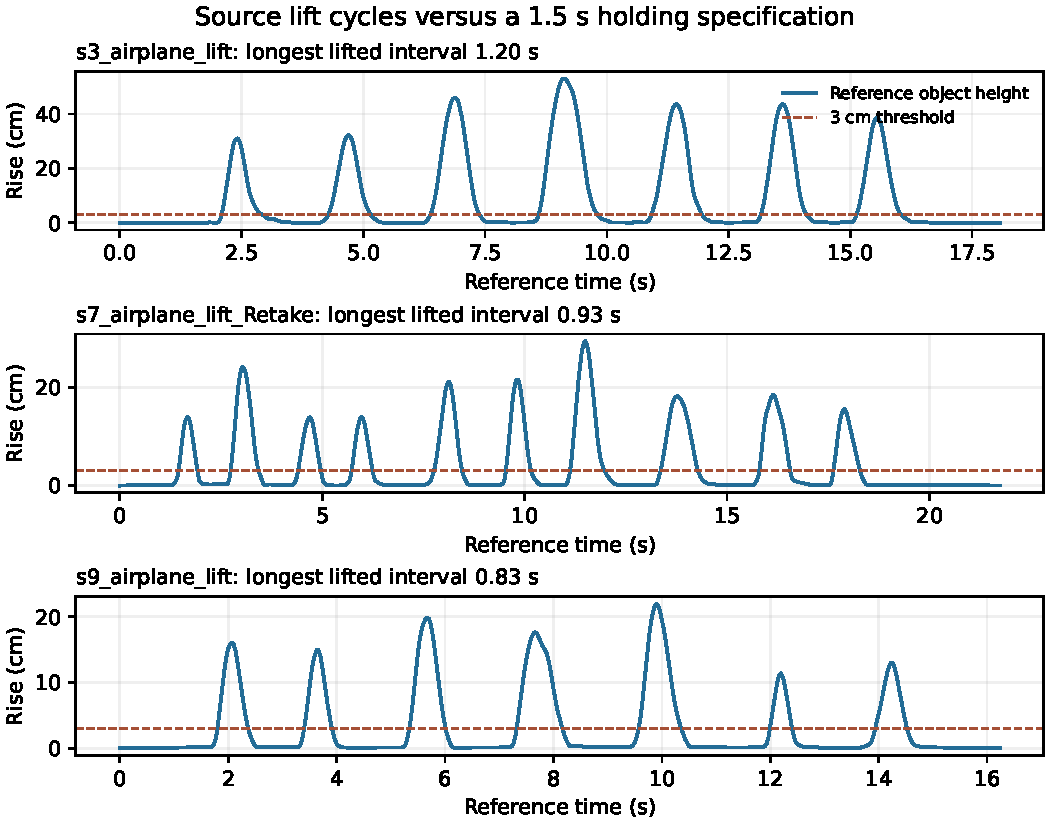
\includegraphics[width=.95\linewidth]{figures/reference_hold.pdf}
\caption{Source object-height targets over reference time. These are labels, not successful physical rollouts. Repeated lift/return cycles are incompatible with requiring perfect tracking and uninterrupted lift lasting 1.5 seconds simultaneously.}
\end{figure}

Eight historical native runs also have no retained success despite 70 stable
instances, including correlated repeats; the new trial has small positive
retained rates. Reference return does not prove the cause of every early drop.
The old gate remains failed. The experiment cannot establish that all predictive
control is useless or that every counted return is accidental object loss.
Repeated corrected states also differ from the first-contact contexts used to
fit this model. Both task specification and closed-loop distribution need attention.

Next we freeze an explicitly synthetic holding task: duplicate 90 raw reference
rows at the maximum height of each FIRST lifted interval, without selecting a
pose using simulator outcomes. The native loader recomputes velocities. A new
actor-only feasibility test asks for 75 consecutive contact-supported physical
steps in that inserted phase, before deliberate release. Generation preserves
initial rows and original remainder; it is not human-data or task-transfer evidence.
No new-task physical result is yet available in this revision.

\section{Limitations and research decision}
These experiments involve one object, three shared motions, two existing actors
and small fixed fitting procedures. Contact proxies plus sampled proximity are
not attributed pairwise forces. Short-horizon measurement is not stable lift,
retention or manipulation utility. No policy training, unseen-object/hand evaluation
or hardware deployment is presented. Optimization seeds do not create independent
physical datasets. Existing papers' claims are not replaced by these diagnostic tests.

The direct learner and tested greedy controller are stopped at their fixed gates.
Before further policy experiments, establish a self-trained baseline on a holding
task whose reference and metric actually agree. A compatible reference is a
prerequisite, not proof of controllable contact or model benefit. The synthetic
plateau feasibility design is frozen separately; current failed data will not
be relabeled as success under a revised metric.

The original user objective remains a journal-level research outcome. This working
paper does not meet it: a distinctive method and consequential matched task evidence
remain necessary. Negative outcomes and the unresolved causal screen are retained
to guide further work rather than converted into positive conclusions.

\section*{Reproducibility}
All new work is isolated in branch \texttt{agent/contact-response-cm}. Original
checkpoints, motion assets and prior evidence are read-only. Physical/differential
code is fixed at \texttt{466e80d}/\texttt{44f22ea}; factorization at
\texttt{bbd5ba4}; fresh collection at \texttt{59de1cf}; null recovery at
\texttt{33d1085}. Randomized collection uses \texttt{510a00e}; direct fitting
\texttt{2075314}; independent auditing \texttt{f283bb9}. Closed-loop task
collection uses \texttt{c0ec955}; task/reference audit and next synthetic task
design use \texttt{b2b26e0}. Manifests preserve commands, input SHA, GPU UUID,
budgets and failures. Every table and reference figure comes from recorded data.
The PDF is a ReportLab review copy; portable LaTeX source and tables are also
retained. Earlier manuscript revisions are preserved separately.

\begin{thebibliography}{9}
\bibitem{he2025} Z.He et al. Scaling Cross-Embodiment World Models for Dexterous Manipulation.
arXiv:2511.01177, 2025. \url{https://arxiv.org/abs/2511.01177}.
\bibitem{xu2025} S.Xu et al. Dexplore:Scalable Neural Control for Dexterous Manipulation
from Reference-Scoped Exploration.2025. \url{https://arxiv.org/abs/2509.09671}.
\bibitem{farahmand2017} A.-M.Farahmand, A.Barreto, D.Nikovski. Value-Aware Loss Function
for Model-based Reinforcement Learning.2017. \url{https://proceedings.mlr.press/v54/farahmand17a.html}.
\bibitem{qiu2026} J.Qiu et al. AD-WM:Action-Discriminative World Models for Counterfactual
Model Predictive Control.2026. \url{https://arxiv.org/abs/2609.30264v2}.
\bibitem{rudolph2024} M.Rudolph et al. Learning Action-based Representations Using Invariance.
2024. \url{https://arxiv.org/abs/2403.16369}.
\bibitem{fey2026} N.Fey et al. Contact-UAN:Unsupervised Actuator Networks as a Residual
World Model for Humanoid Control.2026. \url{https://contact-uan.csail.mit.edu/}.
\bibitem{rakelly2021} K.Rakelly, A.Gupta, C.Florensa, S.Levine. Which Mutual-Information
Representation Learning Objectives are Sufficient for Control?2021.
\url{https://arxiv.org/abs/2106.07278}.
\end{thebibliography}
\end{document}
